\chapter{Исследовательская часть}

В данном разделе будут приведены примеры работы программы, и будет проведен сравнительный анализ реализованных алгоритмов поиска редакционного расстояния по затраченному процессорному времени, а также анализ затрат по памяти.

\section{Технические характеристики}

Технические характеристики устройства, на котором выполнялось исследование приведены ниже.

\begin{itemize}
	\item операционная система: Manjaro Linux \cite{manjaro};
	\item память : 7,6 GiB;
	\item процессор: 8 × Intel® Core™ i5-10210U CPU @ 1.60GHz \cite{intel}.
\end{itemize}

\clearpage

\section{Демонстрация работы программы}

На рисунке \ref{img:example} приведен пример работы программы.

\begin{figure}[H]
	\begin{center}
		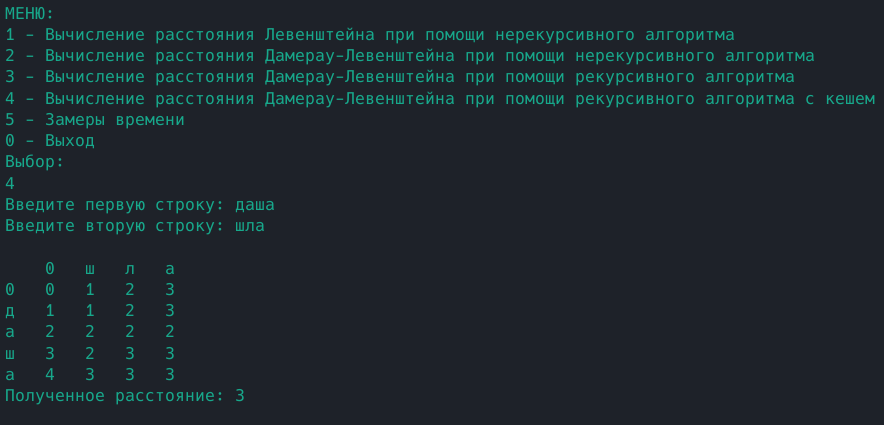
\includegraphics[scale=0.7]{img/example.png}
	\end{center}
	\captionsetup{justification=centering}
	\caption{Пример работы программы}
	\label{img:example}
\end{figure}

\section{Временные характеристики}

Функция process\_time\_ns из библиотеки time языка программирования Python возвращает  процессорное время в наносекундах.

Замеры проводились для длины слов от 1 до 9 на случайных входных строках.

На рисунках \ref{img:dam_lev_rec_vs_matrix}-\ref{img:lev_vs_dam} приведены графические результаты сравнения временных характеристик.

\begin{figure}[H]
	\begin{center}
		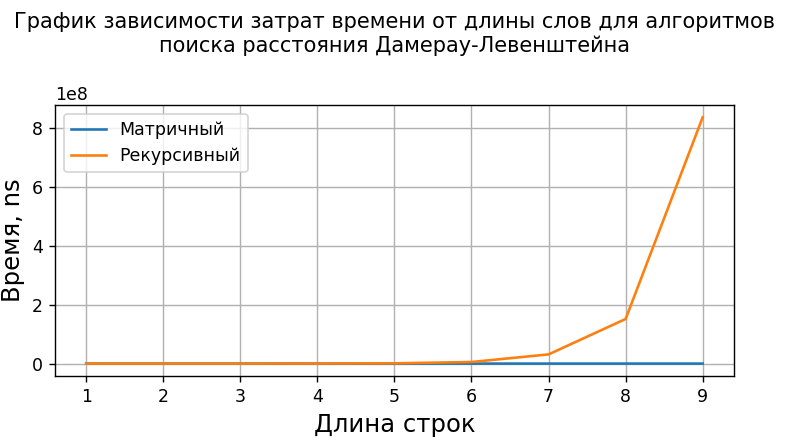
\includegraphics[scale=0.7]{img/dam_lev_rec_vs_matrix.png}
	\end{center}
	\captionsetup{justification=centering}
	\caption{Сравнение по времени рекурсивного алгоритма Дамерау-Левенштейна и матричного алгоритма Дамерау-Левенштейна}
	\label{img:dam_lev_rec_vs_matrix}
\end{figure}

\begin{figure}[H]
	\begin{center}
		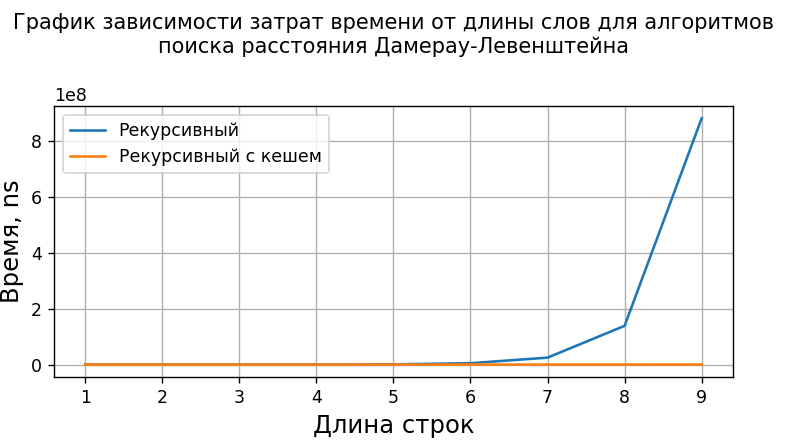
\includegraphics[scale=0.7]{img/dam_lev_rec_vs_cache.png}
	\end{center}
	\captionsetup{justification=centering}
	\caption{Сравнение по времени рекурсивного алгоритма Дамерау-Левенштейна и рекурсивного алгоритма Дамерау-Левенштейна с кешем}
	\label{img:dam_lev_rec_vs_cache}
\end{figure}

\begin{figure}[H]
	\begin{center}
		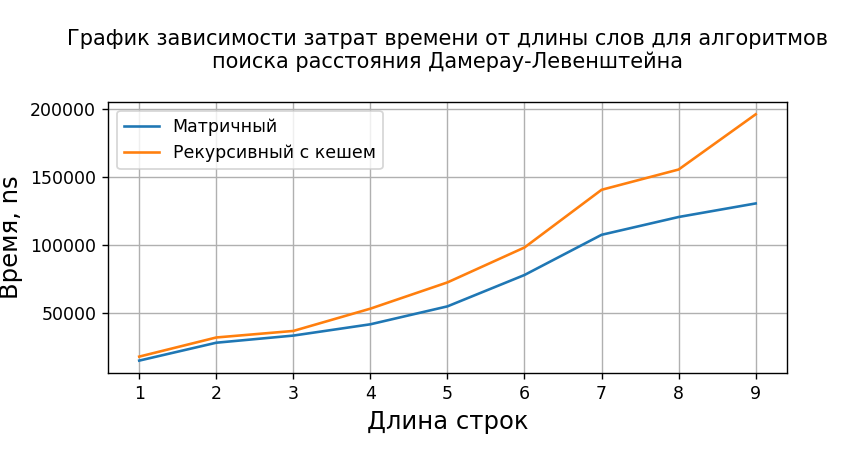
\includegraphics[scale=0.7]{img/dam_lev_cache_vs_matrix.png}
	\end{center}
	\captionsetup{justification=centering}
	\caption{Сравнение по времени рекурсивного алгоритма Дамерау-Левенштейна с кешем и матричного алгоритма Дамерау-Левенштейна}
	\label{img:dam_lev_cache_vs_matrix}
\end{figure}

\begin{figure}[H]
	\begin{center}
		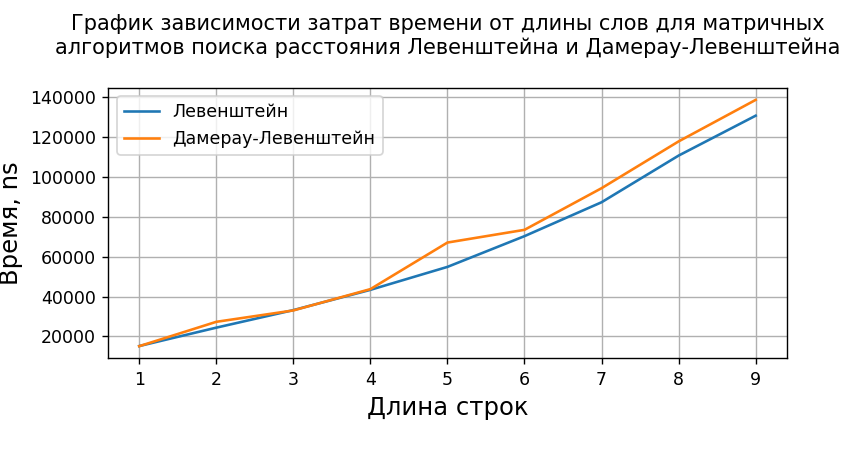
\includegraphics[scale=0.7]{img/lev_vs_dam.png}
	\end{center}
	\captionsetup{justification=centering}
	\caption{Сравнение по времени матричного алгоритма Левенштейна и матричного алгоритма Дамерау-Левенштейна}
	\label{img:lev_vs_dam}
\end{figure}

\section{Анализ затрат по памяти}

Проведем анализ используемой памяти для рекурсивного, матричного и рекурсивного с кешем алгоритмов Дамерау-Левенштейна.

Для рекурсивного алгоритма при каждом вызове происходит выделение памяти под следующие типы данных:

\begin{itemize}
	\item 2 строки типа $str$;
	\item 2 длины строк типа $int$;
	\item адрес возврата - m байт;
	\item 3 или 4 локальных переменных типа $int$.
\end{itemize}

При этом глубина рекурсии равна сумме длин двух строк. Таким образом, используемая память рекурсивного алгоритма в среднем равна:

\begin{equation}
	\label{eq:rm}
	M_{r} = (5,5 \cdot sizeof(int)+2 \cdot sizeof(str)+m)\cdot(|s1|+|s2|)
\end{equation}

Для нерекурсивного алгоритма происходит выделение памяти под следующие типы данных:

\begin{itemize}
	\item 2 строки типа $str$;
	\item 2 длины строк типа $int$;
	\item матрицу с размерами, равными длинам строк, увеличенным на 1;
	\item адрес возврата - m байт;
	\item 3 или 4 локальных переменных типа $int$.
\end{itemize}

Таким образом, используемая память нерекурсивного алгоритма в среднем равна:

\begin{equation}
	\label{eq:mm}
	M_{m} = (5,5+(|s1|+1) \cdot (|s2|+1)) \cdot sizeof(int)+2 \cdot sizeof(str)+m
\end{equation}

Для рекурсивного алгоритма с кешем при каждом вызове происходит выделение памяти под следующие типы данных:

\begin{itemize}
	\item 2 строки типа $str$;
	\item 2 длины строк типа $int$;
	\item ссылка на матрицу $*int$;
	\item адрес возврата - m байт;
	\item 3 или 4 локальных переменных типа $int$.
\end{itemize}

\begin{equation}
	\label{eq:rm}
	M_{1} = (5,5 \cdot sizeof(int)+2 \cdot sizeof(str) + m +sizeof(*int))\cdot(|s1|+|s2|)
\end{equation}

Также перед началом рекурсии выделяется память под матрицу с размерами, равными длинам строк, увеличенным на 1.

\begin{equation}
	\label{eq:rm}
	M_{2} = (|s1|+1) \cdot (|s2|+1) \cdot sizeof(int)
\end{equation}

При этом глубина рекурсии равна сумме длин двух строк. Таким образом, используемая память рекурсивного алгоритма с кешем в среднем равна:

\begin{equation}
	\label{eq:rm}
	M_{rc} = M_{1}+M_{2}
\end{equation}

Алгоритм нахождения расстояния Дамерау-Левенштейна отличается от алгоритма нахождения расстояния Левенштейна только тем, что добавляется операция транспозиции. Поэтому количество локальных переменных для алгоритма Левенштейна будет равно 3. Всё остальное аналогично.

\section{Вывод}
Был проанализирован объем используемой памятия для рекурсивной, матричной и рекурсивной с кешем версий алгоритмов. Можно сделать вывод, что матричные алгоритмы проигрывают рекурсивным, потому что максимальный размер памяти в них растет, как произведение длин строк, а в рекурсивных --- как сумма длин строк. При этом рекурсивные алгоритмы с кешем проигрывают обоим.

Приведенные характеристики времени показывают, что рекурсивная реализация алгоритма сильно проигрывает по времени. В связи с этим, рекурсивные алгоритмы следует использовать лишь для малых размерностей строк. Но рекурсивная реализация с кешем намного быстрее классической рекурсивной реализации, поэтому является более оптимальным вариантом для применения.

Также в результате эксперимента было установлено, что алгоритм Дамерау-Левенштейна работает медленнее Левенштейна из-за дополнительной операции.